\setmainfont{Noto Serif}
\setsansfont{Noto Sans}
\setmonofont{Noto Sans Mono}
\setstretch{1.35}

\section{Правила Вудворда-Хоффмана}
1С. Постройте корреляционную диаграмму образования хюккелевской системы, имеющей строение треугольной призмы, из двух одинаковых треугольных хюккелевских систем. Определите чему равно изменение полной электронной энергии в ходе данной реакции. Используйте базис $1s$ атомных орбиталей.
\par
\begin{wrapfigure}{r}{28mm} %this figure will be at the right
    \centering
    \vspace{-1mm}
    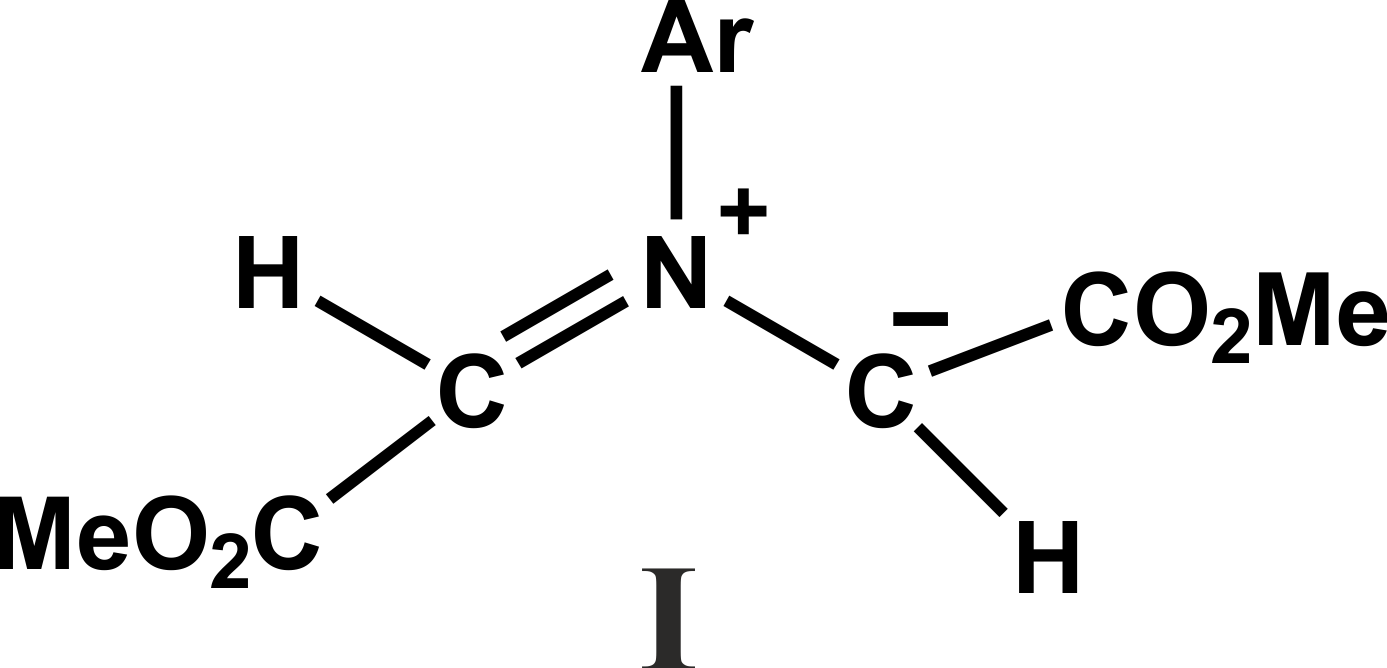
\includegraphics[width=28mm]{images/Fig_2_1_2.png}
    \vspace{0mm}
\end{wrapfigure}
2К. Определите по какому механизму (кон- или дисротаторный) протекает реакция термической циклизации транс-азометинового илида I, изображенного на рисунке. Укажите стереохимию продукта реакции и постройте корреляционную диаграмму. Соединение I изоэлектронно аллил-аниону, $\text{Ar}=\text{C}_6\text{H}_4-\text{OCH}_3$.
\par
%$\leftrightarrows$
3. Постройте корреляционную диаграмму цис-транс-изомеризации производных этилена.
\par
4С. Постройте корреляционную диаграмму реакции термического циклоприсоединения бутадиена и этилена в $4\pi_s$ + $2\pi_s$ топологии. Используя правила Вудворда-Хоффмана рассмотрите протекание реакции в других топологиях. Можно ли в этих случаях построить корреляционную диаграмму?
\par
5Т. Каким образом протекает реакция $\text{H}_2$ + $\text{D}_2$ $\rightleftarrows$ 2$\text{HD}$:  термически или фотохимически? Постройте корреляционную диаграмму.
\par
\begin{wrapfigure}{r}{34mm} %this figure will be at the right
    \centering
    \vspace{-1.9mm}
    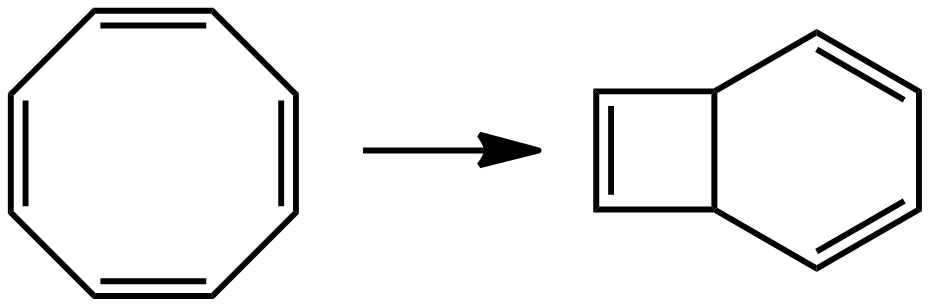
\includegraphics[width=28mm]{images/Fig_2_1_5.png}
    \vspace{-3.4mm}
\end{wrapfigure}
6С. Постройте корреляционную диаграмму изомеризации  циклооктатетраена по дисротаторному механизму согласно реакции, приведенной на рисунке. Может ли данная реакция протекать термически?
\par
\begin{wrapfigure}{r}{34mm} %this figure will be at the right
    \centering
    \vspace{-1mm}
    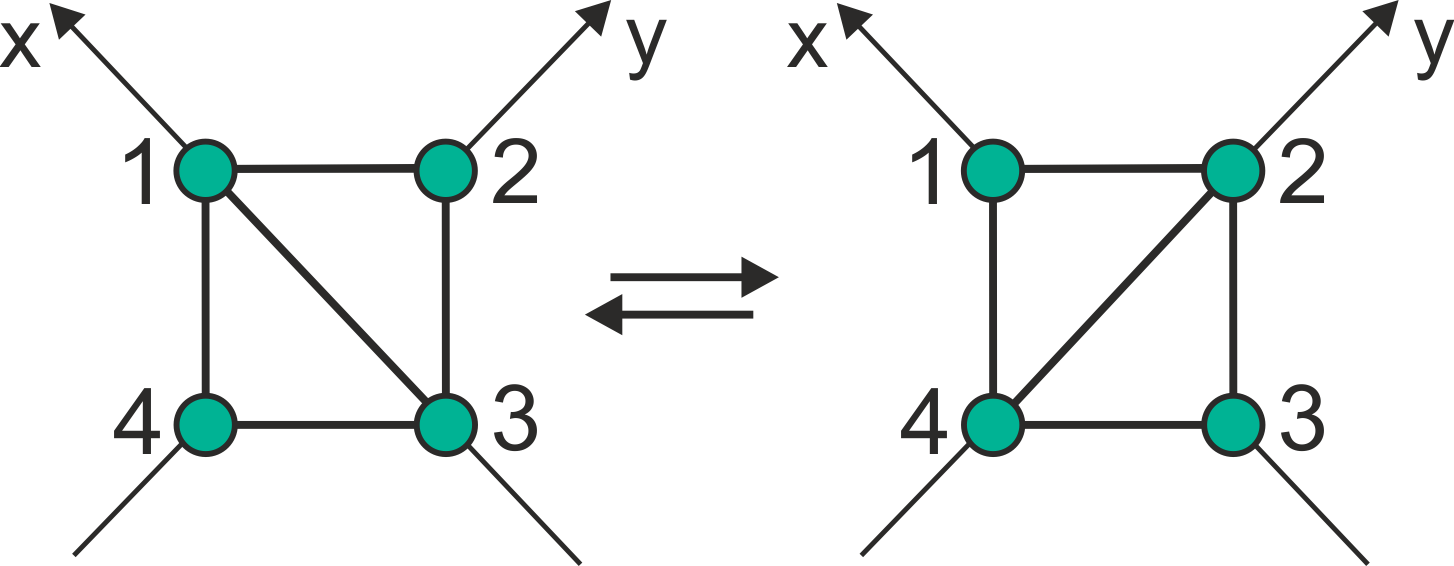
\includegraphics[width=34mm]{images/Fig_2_1_7.png}
    \vspace{-3.5mm}
\end{wrapfigure}
7. Постройте корреляционную диаграмму реакции изомеризации, изображенной на рисунке справа. Разрешена или запрещена данная реакция при термическом протекании? Чему равно изменение полной электронной энергии в ходе данной реакции?
\par
8Т. Сформулируйте правила Вудворда-Хоффмана для реакции циклоприсоединения Дильса-Альдера в общем случае.
\par
9. Определить термически или фотохимически разрешена реакция присоединения атома водорода к молекуле водорода. Предполагается образование циклической молекулы при сближении $\text{H}$ и $\text{H}_2$ перпендикулярно направлению связи $\text{H}$$-$$\text{H}$. Определите симметрию молекулярных орбиталей продуктов и~реагентов реакции в терминах неприводимых представлений сохраняющейся группы симметрии. В случае фотохимического механизма предварительно определить, разрешен ли электрический дипольный переход в предполагаемое возбужденное состояние.
\par
\begin{wrapfigure}{r}{17.5mm} %this figure will be at the right
    \centering
    \vspace{-3mm}
    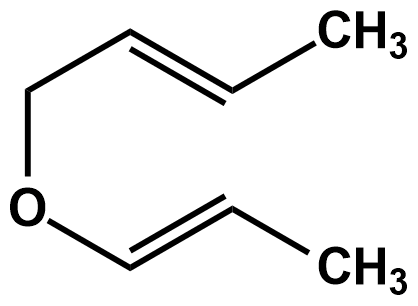
\includegraphics[width=17.5mm]{images/Fig_2_1_10.png}
    \vspace{-5mm}
\end{wrapfigure}
10С. Исходя из правил Вудворда-Хоффмана опишите механизм протекания [3,3]-сигматропного сдвига (перегруппировка Кляйзена) в производном 2,6-октадиена, который изображен на рисунке, в случае ее термического протекания. Укажите стереохимию продукта реакции.
\par
11. Определите разрешена ли реакция присоединения $\text{N}$$-$$\text{H}$ к $\text{H}$$-$$\text{H}$ с образованием NH$_3$? Сближение происходит так, что связи $\text{N}$$-$$\text{H}$ и $\text{H}$$-$$\text{H}$ перпендикулярны друг другу. Для атома азота учитывайте только $2p$ атомные орбитали.
\par
12. Реакция циклоприсоединения двух молекул этилена в супра-/супра- топологии запрещена термически. Может ли металл в конфигурации $d^n$ снять этот запрет? Чему равно минимальное и максимальное значение $n$?
\par
13К. Постройте корреляционную диаграмму термического превращения циклооктатетраена в кубан в супра-\,/\,супра- топологии.
\par